\chapter{Literature Review}
%\label{sec:ob_rel}
\section{Introduction to water quality control}
\subsection{Automated system for water quality control}
%%%%%%%%%%PLC and some real application cases in WTP
%Explain PLC better by \cite{WasteWaterTreatment2018}
%re organize this section
Programmable logic controller (PLC) is an industrial computer system designed for any process requiring a series of devices and equipment operates cohesively to achieve multiple purposes in manufacturing or treatment processes. The main components of PLC include a center process unit (CPU), input modules and output modules (I/O). CPU is responsible to process digital signals from input modules and send commands through output modules based on the control logics programmed on the PLC. For chemical dosing control in water treatment plants (WTPs), PLC system receives readings from turbidity and pH sensors and uses pumps to dose aluminum solution automatically \citep{andhareSCADAToolIncrease2014}. The PLC system with the capability of producing real-time output commands in response to the input sigals also makes it widely used in the wastewater treatment plants (WWTPs). For oxygen concentration control in the aeration tank, PLC system receives signals of dissovled oxygen (DO) detectors and transmits signals to open or close the electric butterfly valves to further alter the DO concentration \citep{zhuApplicationPLCSewage2017}. Although PLC systems are the most used system across industries for its easy programming and reliable control, PLC system is merely a device that can be programmed to control operative devices with on-off logic (i.e., a logic control with two states) and the capability of complex control is compromised. In reality, many WTPs or WWTPs have the need of precise control of the treatment processes. Being awared of the limitations of the PLC systems, a more advanced controller called proportional–interal–derivative (PID) controller for receiving analog signals was developed to obtain more sophisticated controls over the operative devices.

%%%%%%%%%%PID and examples
%PID control is used where greater levels of precision in control are required. It combines three control terms to give a single output to drive the setpoint. 
To react to rapidly-changing process conditions, a PID controller generates an output value based on continuous calculation of an error value e(t) as the difference between a desired setpoint (SP) and a measured process variable and applies a correction based on proportional, integral, and derivative terms. The use of the "P", "I", and "D" allows the system to quickly reach steady state with a feedback control system (i.e., the system output is returned to the system input which is included in the decision making process in PID controller). Generally speaking, a PID controller is a technology (i.e., a specialist algorithm) for contorlling a single device with more complex logics, while a PLC system is a physical system consists of different modules and capable of controlling dozens of devices only with two-state logic. In addition, A PID controller can be designed to operate on PLC device and provide a more precise control strategy to a designated device. In WWTPs, a single-variable feedback analog control loop in PID can be used to control the temperature in the activated sludge treatment by stablizing the system temperature in a shorter time \citep{badosDesignPIDControl2020}. The feedback control scheme is also applied in WTPs to adjust the addition of chlorine dosage (i.e., also known as the disinfection process, chlorination, or postchlorination) to reach the target concentration of free chlorine residual (FRC) \citep{wangCompositeControlPostChlorine2019}. Disinfection process is carried out in a chlorine contact tank which provides sufficient time for chlorine to disinfect pollutants. Since the chlorine added by the dosing device requires time to travel from the entry to the exit, the system output can only reflect the changes of water quality in a delayed time of 30 minutes (i.e., the designed time for water to travel in chlorine contact tank is usually 30 minutes or longer). In the case of chlorination, the lag of time makes feedback control difficult \citep{kobylinskiLineControlStrategies2006} as the system is delayed in responding to any sudden surge of the pollutants when it can only receive output at the end of the disinfection process. PID controllers in WWTPs also encounter similar challenges as the increasing complexity of water quality and stricter regulations on the discharged water quality. 

%%%%%%%%%%Transition to how the algorithms in PID can be replace by AI, ML, 
%Introduce to MPC, feedforward control in comparison with PID controller
%The use of mathematical modeling is not ideal, turning to the use of AI modeling
To tackle the difficulties encountered in process control system, many control strategies are proposed, such as feed forward-feedback control, linearized and optimal control, model-predictive control, and fuzzy control, etc \citep{demirFeedbackControlChlorine2014a}. Among the algorithms used in control strategies, Artificial Intelligence (AI) modeling has gained the most attentions in recent years compared to modeling based on mathematical models or empirical formulas. In WTPs or WWTPs, to fully understand the physical, biological, and chemical interactions in the treatment plants is very difficult. The unpredictable behaviors during the water treatment can be the significant changes of influent flow rate, flucutations of water quality, the complexity of biological treatment process, and the large time delay exists between this control variable and the process input, etc. Therefore, AI modeling shows a great potential in dealing with the highly complex conditions in the treatment process \citep{liRecentAdvancesArtificial2021}. In the next sections, the applications of different AI modeling methods will be discussed.

\subsection{Artificial Intelligence}
%AI include fuzzy logic, a subset of ML. ML includes SVM, a subset of DL. DL includes LSTM.
Artificial intelligence (AI) can perform cognitive tasks with the development of computational solutions. The concepts of AI are usually confused, in fact, AI is a very broad term and any kind of algorithms or models which involved in decision-making with computation fall in the domain of AI. For example, fuzzy logic and optimization algorithm are formulated with human design and computer decision making process. There are another subset of AI called machine learning (ML), but the process of generating a ML model is different to generating a fuzzy logic model. ML uses learning algorithms to generate a model via learning from historical or large amount of data without being explicitly programmed. ML algorithms can be classified into three categories, which are Supervised, Unsupervised, and Reinforcement learning. In the training process of supervised learning, input variable (x) and output variable(Y) we will provided, and model will learn from the provided dataset to map the x to the Y. A trained supervised model can generate a prediction for the response to the new data (i.e., also called the unseen data). Unsupervised learning is when the dataset is not labelled, the model can learn to infer patterns in the dataset without reference to the known outputs. This type of algorithm can find similarities and differences in the data. In reinforcement learning, models are designed to constantly interact with the environment in a try-and-error way and recieved rewards and punishments based on the purpose of the tasks. Generating a optimal action to achieve lowest penalties is the main function of a reinforcement learning model. In process control, supervised learning are frequently used in many senarios.

Regression is a supervised machine learning technique used to predict continuous values. A regression model can estimate the relationship between the input variables in the system and the output target from a given dataset, and then use the nonlinear relationship to map the unseen input data to a predicted output data. This type of application is sutiable for water quality prediction  \citep{librantzArtificialNeuralNetworks2018}, and sensor fault detection \citep{cecconiSoftSensingOnLine2021}, etc. 

Fuzzy logic (FL) control is still an effective strategy for process control, and this type of AI modeling is called reasoning. Fuzzy logic is described as an interpretative system in which objects or elements are related with borders not clearly defined, granting them a relative membership degree and not strict, as is customary in traditional logic. The typical architecture of a fuzzy controller, shown in Figure 3, consists of a fuzzifier, a fuzzy rule base, an inference engine, and a defuzzifier \citet{santinFuzzyControlModel2015} proposed a hybrid control system comprised of FL controller and model predictive control using optimizaion model to control the chlorine dosing in a WTP. FL controller and optimzation model fall in the domain of AI, which is excluded from the subset of ML.

Fuzzy logic (FL), a method based on multi-valued logic, uses fuzzy sets to study fuzzy judgement, which allows FL-based fuzzy inference systems to simulate the human brain to implement natural inference [40].The adaptive fuzzy neural inference system (ANFIS) composed of FL and ANN with an inference mechanism has high interpretability compared to common ANN. The combined model has been used to control coagulant dosing systems [41,42].

\subsection{Machine learning and deep learning}
In machine learning, popular models which are frequently used by the researchers for training predictive models are Supporting Vector Machine (SVM), Random Forest (RF), and Artificial Neural Networks (ANN). \citet{librantzArtificialNeuralNetworks2018} trained a RF model to predict the free residual chlorine concentration (FRC) in a WTP, and \citet{xuAlternativeLaboratoryTesting2021} built a RF-based model to predict total nitrogen concentration in water bodies. \citet{guoPredictionEffluentConcentration2015} compared the reliability and accuracy of an ANN model and a SVM model in predicting 1-day interval T-N concentration in a WWTP, and the results showed that RF model has higher accuracy while ANN model is more reliable for assisting decision-making process.

As the the computing power doubled every 18 months according to Moore's law. A subset of ML, Deep Learning (DL) becomes more accessible for sovling everyday issues. In simplicity, DL models can be defined as neural networks with more than two hidden layers (i.e., the model complexity increased and required more computing power to calculate). In DL, there are various types of architectures designed based on the type of problems. For image processing, Convolutional Neural Network (CNN) is designed to extract important features from the image vectors. Another popular DL architecture is Recurrent Neural Network (RNN), which is powerful in solving time series-related applications and Natural Language Processing (NLP) tasks \citep{liERNNDesignOptimization2018}. Although each architecture has their strengh in tackling different types of problems, both architectures can be used for a single task \citet{liPredictionFlowBased2022} built a regression CNN-RNN model for rainfall-runoff prediction. DL can be extremely powerful when multiple architectures ared fused into a single model to perform a specific task, which cannot be realized by machine leraning models. That being said, DL can achieve higher model performance in terms of the prediction accuracy compared to ML. 

\section{Water quality control with machine learning}
%%it's better to find papers that can provide comparison between DL and ML or traditional models
\subsection{Drinking water treatment plants}
%Background
A drinking water treatment plant (DWTPs) produces potable (i.e., drinking water) water for human consumptions by removing contaminants from the source water, such as lake or stream, or from an underground aquifer. The raw water enters DWTPs and goes through treatmet units of coagulation, flocculation, sedimentation, filtration, and disinfection in sequence as the primary treatment scheme in the conventional DWTPs \citep{liRecentAdvancesArtificial2021}. 
%detailed functions of the treatment process
%1.8.1 Drinking Water Treatment Drinking water treatment plant could be classified into: – Disinfection plant which is used for high-quality water source to ensure that water does not contain pathogens – Filtration plant: this is usually used to treat surface water – Softening plant which is used to treat groundwater Typical filtration plant is shown in Fig. 5 which is designed to remove odors, color, and turbidity as well as bacteria and other contaminants. Filtration plant employs the following steps: a.Rapid mixing : where chemicals are added and rapidly dispersed through the water b.Flocculation : Chemicals like alum (aluminum sulfate) are added to the water both to neutralize the particles electrically and to make them come close to each other and form large particles called flocs that could more readily be settled out c.Sedimentation : During sedimentation, floc settles to the bottom of the water supply, due to its weight d.Filtration: Once the floc has settled to the bottom of the water supply, the clear water on top will pass through filters of varying compositions (sand, gravel, and charcoal) and pore sizes in order to remove fine particles that were not settled, such as dust, parasites, bacteria, viruses, and chemicals e.Disinfection : involves the addition of chemicals in order to kill or reduce the number of pathogenic organisms
During the treatment processed, colloids, suspended matter, pathogenic microorganisms and organic matter are removed to meet the regulated standard. However, the quality of raw water isn't always stable, and corresponding actions are required to be promptly adopted when events like the surge of pollutants or the large variability of the influent flow. In any event, the treated water from DWTPs should generate drinking water which complies the World Health Organization's Guidelines (WHO's guideline) for drinking water quality. Otherwise, the treated drinking water should either be discharged and result in the short term outage of water supply to the downstream cities or the users will receive contaminated drinking water which can potentially transmit diseases and cause illness.

%Turbidity
Turbidity is one of the critical water quality indicators, which can be defined as the "optical quality" of water, and the unit to decribe the turbidity is called Nephelometric Turbidity Unit (NTU). High levels of turbidity in raw water can impede the effectiveness of filtration and chlorination processes, and potentially cause short-term outages of water supply. Heavy rainfall and fissures within the aquifer can also lead to turbidity events are mostly likely to cause high turbidity \citep{worldhealthorganizationWaterQualityHealth2017}. The challenge in event of high turbidity in raw water is it occurs rapidly and mitigating activities must be actionable immediately. To address sudden event of such, \citet{stevensonAdvancedTurbidityPrediction2019} trained forecasting models based on general linear model (GLM) and RF to predict the time when the turbidiy reaches higher than 7 NTU. The results indicate both model can successfully predict the events (i.e., with accuracy between 0.81 and 0.86), and RF model is found to have higher precision due to it's ability to capture the nonlinear relationship between rainfall (mm) and turbidity (NTU).

%Coagulation dose
To maintain operational costs and water quality in the coagulation process, the amount of coagulant, which is mainly subject to the turbidity and alkalinity in the raw water, is traditionally determined thourgh manually sampling and analysis. Jar test is designed to find out the optimal chemical dosage for coagulation to remove the turbidity in raw water, and the entire process includes on-site sampling and up to more than 40 minutes of laboratory works \citep{ganiEffectPHAlum2017}. To replace the laborious procedure of jar tests, \citet{wangIntegratingWaterQuality2022} proposed using principal component regression (PCR), support vector regression (SVR), and long short-term memory (LSTM) neural network to build predictive models for outputing daily estimated chemical dosage. Compared with linear PCR model, nonlinear SVR and LSTM models captures more relationship between the chemical dose (e.g., ferric sulfate) and the raw water quality based on a higher R-squared value of 0.70.

%membrane-filtration modeling

%Disinfection
Disinfection is the last step of water treatment processes in drinking water treatment plants to generate safe potable water. In this step, one or more chemical disinfectants like chlorine, chloramine, or chlorine dioxide are added into the water to inactivate any remaining pathogenic microorganisms. However, the chlorination process requires precise dosing of disinfectant---too high will lead to the formation of disinfection byproducts (DBPs), and too low will result in insufficient levels of the residaul disinfectant concentration. In both senarios, the treated drinking water can pose health threats to the end users. The aforementioned PID controller can achieve automatic dosing of disinfection, however, \citet{wangModelPredictiveControl2020} found out that the accuracy of the predicted disinfectant dosage using (i.e., chlorine is used in this paper) a Support Vector Regression (SVR) model outperformed a PID controller in both simulation and experimental conditions. An Artificial Nerual Network based model also shows a more satisfied cost reduction in a chlorination dosing control system comapred to PID controller \citep{librantzArtificialNeuralNetworks2018}.

%DBPs
The invariability of the raw water quality is always a big issue for disinfection. For instance, chlorine dose can be excessive dosed when the treated water contains less pollutants (e.g., non-organic matters and ammonia nitrogen). Exessive addition of chlorine results in the problem of wasting chemicals which is reflected on the increase operational cost and potentially generate undesired disinfection by-products (e.g., trihalomethanes (THMs), which are carcinogenic to human) due to the chemcial reaction between pollutants and overly dosed chlorine. \citet{xuUsingSimpleEasy2022} trained an ANN model for predcting the occurrence of THMs in tap water using simple and easy water quality parameters (e.g., pH, temperature, $UVA_{254}$ and residual chlorine ($Cl_{2}$)). Despite the results showed a good model accuracy in predicting for THMs (i.e., T-THMs, TCM and BDCM), the applications of the model is largely limited in reality due to the lack of dataset regarding the quantity and quality . In fact, lack of high quality dataset for trianing ML models is a common issue, which explains up until recently, mathametical or empirical based AI models like fuzzy logic \citep{gamizFuzzyGainScheduling2020,godo-plaControlPrimaryDisinfection2021} is still widely used for process control in WTPs.

\subsection{Wastewater treatment plants}
%Background
Human activies produce wastewater and discharge from homes, businesses, factories and commercial activities to the sewage systems which connect to wastewater treatment plants (WWTPs). The function of a WWTP is to remove contaminants from sewage and water so that the treated water can be returned to the natural water body without dangering any living beings reside in the ecosystem. Undertreated wastewater can lead to harmful algal blooms or cause oxygen deficit in the water (i.e., low oxygen content can kill the fishes). The steps for treating municipal wastewater involve three major categories---primary treatment, secondary treatment and tertiary treatment. The pollutants which will either float or settle will be removed in primary treatment; next, secondary treatment is mainly responsible for removing BOD$_5$ in the biological processes; in the final tertiary treatment, membrane filtration, adsorption by activated carbon and addition of disinfectant can be applied optionally to futher eliminate the undesired pollutants in the water.

%Introduce the need of process control
Wastewater can be defined as the flow of used water discharged from homes, businesses, industries, commercial activities and institutions which is transported to treatment plants via pulbich sewer system or engineered network of pipes. This wastewater is further categorized and defined according to its sources of origin. Domestic wastewater refers to water discharged from residential sources generated by kitchen wastewater, cleaning and personal hygiene. Industrial/commercial wastewater is generated and discharged from manufacturing and commercial activities, such as textile industry and food and beverage processing wastewater. Institutional wastewater characterizes wastewater generated by large institutions such as hospitals and educational facilities. Regardless of the source of the wastewater, WWTPs have to achieve at least three sustainability targets: environmental protection (i.e., low pollutants discharge), social acceptance (i.e., human sanitary protection) and economic development (i.e., feasible operational and management costs) \citep{manninaDecisionSupportSystems2019}. To effectively achieve these goals, process control is requried to reduce energy consumption, improve on effluent quality, and save costs in plant operation and management. The focus of this study is on discussing the development of using process control for treatment operation and management.

%Examples of using predicted water quality for process control
Under known operational conditions of a WWTP, machine learning models can be trained to assist the plant operators optimize treatment processes to improve effluent quality . \citet{wangMachineLearningFramework2021} proposed a machine learning framework, utilizing a model based on Random Forest to predict the effluent Total Suspended Solid (TSS) and phosphate (PO$_4$). This study features using collected data from six on-line sensors (i.e., flow rate, TSS, pH, PO$_4$, temperature, and total solids (TS) meters) across the treatment line to train the RF model. The results indicated that the influent temperature is the most influential variable for both TSS and PO$_4$ in the effluent, and PO$_4$ depends strongly on the TSS in aeration basins, etc. It has been suggested that the combined use of RF model and analytical tools allows the author to pinpoint the critical factors influencing on the effluent quality, and this seems to be a innovative approach. However, there are severl major drawbacks hindering such model developments using on-line sensors to collect training data. Many of the existing WWTPs and DWTPs are not equipped with on-line sensors, and lack of automation and instrumentation is common. One of the examples that lack of data from on-line sensor is an emerging techology called aerobic granular sludge (AGS) in secondary treatment (i.e., biological treatment). In addition, \citet{wilenMechanismsGranulationActivated2018} claimed that the complex nonlinear relationships between the sludge, wastewater quality and operational conditions makes the operation and management of AGS difficult. Awaring the high complexity of the AGS and the unavailabilities of on-line sensors, \citet{zaghloulDevelopmentEnsembleMachine2021} attempted to address the issues by collecting data from lab-based reactors and training machine learning models. Considering the intricacy of operation coditions and the AGS system, the author claimed that with the use of feature selection and ensemble model, which is train with three different ML models, overfitting can be prevented. Given that the findings in this study provided good model performance in predicting Chemical Oxygen Demand (COD) and other sludge-related parameters, the results stating the fact of reducing overfitting using ensemble learnings should be treated with caution. Similar to the AGS system, electrocoagulation reactor is also an complex system that the operation and management are based on pH value, the current density, flow rate and the initial concentration of heavy metal ions, etc. Interestingly, instead of using an ensemble model to prevent the overfitting issue claied by \citet{zaghloulDevelopmentEnsembleMachine2021}, \citet{zhuPredictionMethodElectrocoagulation2021} used a deep learning Long and Short-term model (LSTM) and a error compensate Autoregressive Integrated Moving Average model (ARIMA) to predict the removal rate of heavy metal ion concentration in wastewater. A LSTM-ARIMA model has strengthed the model performance compared to solely used LSTM or ARIMA model in predicting removal rate shown by the Results. A possible rationalization of using as LSTM model without worrying model overfitting is that deep learning is sophsiticated enough for learning the nonlinear patterns in complex system while machine learning model like RF might fail to capture the intricate relationships, resulting in overfitting.

%The challenge of using sensors in process control
The advancement in technology allows the easy access to real-time water quality data via on-line sensors. The collected real-time data can be used to train predictive models and assist the plant operation and management. Depite the advantages of what on-line sensors are capable of, the pitfalls can jeopardize the quality of predictives models or even induce wrong decisions for plant operation, ultimately deteriorate treatment efficiency in WWTPs. \citet{haimiShallWeUse2015} suggested that reliable and moderately-priced real-time sensors are not always available, in addition, sensor malfunctions (i.e., fouling or erroneous measurement) can cause the down-time of the sensors. For the unavaible sensors (i.e., "hard-to-measure" or expensive sensors), many research works have proposed building "soft sensors". Instead of using hardware sensors to measure the water paratmers, soft sensor generates real-time values through a machine learning model, which is trained by other easy-to-measure water quality data. In the works of \citet{wangExplicitInterpretableNonlinear2019}, easy-to-measure variables such as, pH, flow rate, TSS, and ammonium nitrate (NH$_4$-N) are input to machine learning models to predict hard-to-measure water quality paratmers of COD and total phosphate (TP). \citet{pattnaikMachineLearningBased2021} also used DO, pH, conductivity, turbidity, and temperature to train a model to predict BOD. It's beleived that both research works can solve the issues of the uavailability of certain water quality sensors. 

%The explanation of what are sensor fouling
The automated treatment operation and management heavily relies on the reliability of the on-line sensors, thus, preventing and the early detection of when the sensors are malfunctioned is the upmost concern to the plant operators. Sensor fault detections can be catogorized into three groups, which are (1) individual faults---an outlier data which can be distinguished with the respect to others data points; (2) contextual faults---an anomalous instance in a specific context and normal in another; (3) collective faults---a cluster of irregular intances with respect to other data trends \citep{chandolaAnomalyDetectionSurvey}. Many research papers have proposed using machine learning models to help identify the sensor fouling.

%Solving sensor fouling-regrssion
Two main types algorithms, which is regression and classification can be used for finding fouling signals. A regression algorithm can identify fouling signals by comparing model predicted outputs (e.g., ammonium or COD concentration) to the actual signals; a classification algorithm can distinguish fouling signals through the direct outputs of the model (i.e., the model outputs 2 class labels, one can be assigned as normal and the other is abnormal signal). \citet{cecconiSoftSensingOnLine2021} proposed a ammonium fault detection mechanism, utilizing a regression ANN model, along with principal component analysis (PCA) and Shewhart monitoring charts (i.e., statistical control chart). The remarkable idea from this study is to analyze the residaul between the predicted ammonium and the real ammonium snesor signal and identify the individual and contextual faults with the help of statistical tools. Despite the accuracy of fault detection mechanism can reach R$^2$ value of 0.87, the method comes with great limitations. The author points out to maintain the high accuracy of the predictive model, the quality of the input data needs to be carefully attended by performing manual cleaning procedures on a weekly basis. 

%sovling sensor fouling-classification
Research has tended to focus on solving collective faults in sensor fault detection (ref of soft sensor solving individual faults) rather than collective faults. The major reason is collectives faults are hidden in regular signals, and only by identifing a combination of signals by experts can spot the irregularity. Thus classification technique using deep learnig is proposed to address collective faults in the works of \citet{mamandipoorMonitoringDetectingFaults2020}. It is believed that this is the first research paper using a LSTM network to achieve a fully automatic fault detection method in WWTPs. Contrast to others works, input variables for model training heavily relies on the manual selection of the experts before inputing into models like PCA and fuzzy nerual networks. The significance of using a deep learning network is it's capability of capturing long-term temperol dependencies from a large dataset compared to machine learning models (i.e., PCA-SVM model). The results showed that the accuracy (i.e., F1-score) from LSTM model is 92\%, outperformed the PCA-SVM model of 87\%. This finding suggests using DL models in classification problems is promising for solving collective faults.

\subsection{Water reclamation system}
%Background
The increasing demands of water in cities is mainly attributed to the rapid urbanization and the population moving from rural to urban centers. In many major cities, the evergrowing water usage and wastewater discharge drive the development of water reclamation \citep{lyuWastewaterReclamationReuse2016}. In WWTPs, the technologies applied in water resue include disinfecting with chlorine addition, ultra-violet (UV) irradiation, biological treatment, and membrane filtration, etc \citep{norton-brandaoReclamationUsedUrban2013}. However, even with the most advanced water treatment technology, the treated reclaimed water quality is still subject to the variability and varations of pollutant contents in wastewater effluent \citep{chenAssessingWastewaterReclamation2003}, and can potentially fail to meet the reclaimed water standard. The research studies propose to apply machine learning techniques to assist the disinfection process in water reclamation can be catogorized into three groups (1) optimize the treatment management in WWTPs to alleviate the loadings of water reclamation process \citep{al-ghazawiUseArtificialNeural2021,vietEnhancementMembraneSystem2021}; (2) actively branch out the desired and undesired wastewater effluent for subsequnt disinfection process of water resue or direct disposal into water body \citep{chenAssessingWastewaterReclamation2003}; (3) adapt process control methods to stablize the disinfection performance in the reclaimed water system \citep{demirFeedbackControlChlorine2014a}. 

The technology advancement and research studies of water reuse have been discussed for more than two decades. However the reseach publications aim at improving the reclaimed water system as a whole in recent years are not too many. The economic reasons behind constructing water reuse facilities universally could be the major obsticle for the government sectors. The economic burden of both building new reclaimed water institution on new locations or retrofit existed WWTPs is deterrent \citep{adewumiTreatedWastewaterReuse2010}. To discover more values and resuable resources from water reuse, \citet{chojnackaTransitionConventionalIrrigation2020} takes the circular economy perpective into accelearting the process of adopting water reuse system for agriculture production. The author introduces the potential of gradually replacing chemical fertilizers with partially treated wastewater for sustainable crops production despite there are many limitations to be overcome. In Italy, the circular concept is also studied by \citet{colellaChallengesOpportunitiesMore2021}. Four different resource recovery senarios were brought up and two of the senarios include the nutrients recovery turned into nitrogen and phosphorus fertilizers. Several researchers in recent years have provided the overall potential and challenges of treated wastewater reuses in the world, it is believed the day of using reuse water universally will soon advant with the collaboration across different disciplines. 

\citep{kehreinCriticalReviewResource2020}
%supplement 

\section{Tools and techniques for enchancing the performance of machine learning modeling}
\subsection{Programming languages}

Matrix Laboratory (Matlab) is a propreitary programming and numeric computing platform used across industries and academia for data analysis, algorithm developments and model buildings. In wastewater treatment industry, Matlab is known for using with an add-on software called Simulink for modeling, simulating, and analyzing the dynamic system (i.e., chemically enhanced primary clarifier \citep{bachisModellingCharacterizationPrimary2015}. The use of Matlab-Simulink in wastewater treatment industry is known for the development control strategries of WWTP automations. In 1987, International Water Association (IWA) developed the first mathematical model for simulation-based evaluation, which is Activated Sludge Model 1 (ASM 1), and the modified activated sludge models and Benchmark Simulation Models (BSM) were further developed in the following years \citep{talibModelingControlWastewater2011}. The difference between the two is, ASM is designed for developing control strategies exclusively in activated suldge treatment process, and BSM 1 is to develop the automation in the entire WWTP \citep{ballhysaWastewaterTreatmentPlant2020}.

\begin{figure}[h]
   \centering
   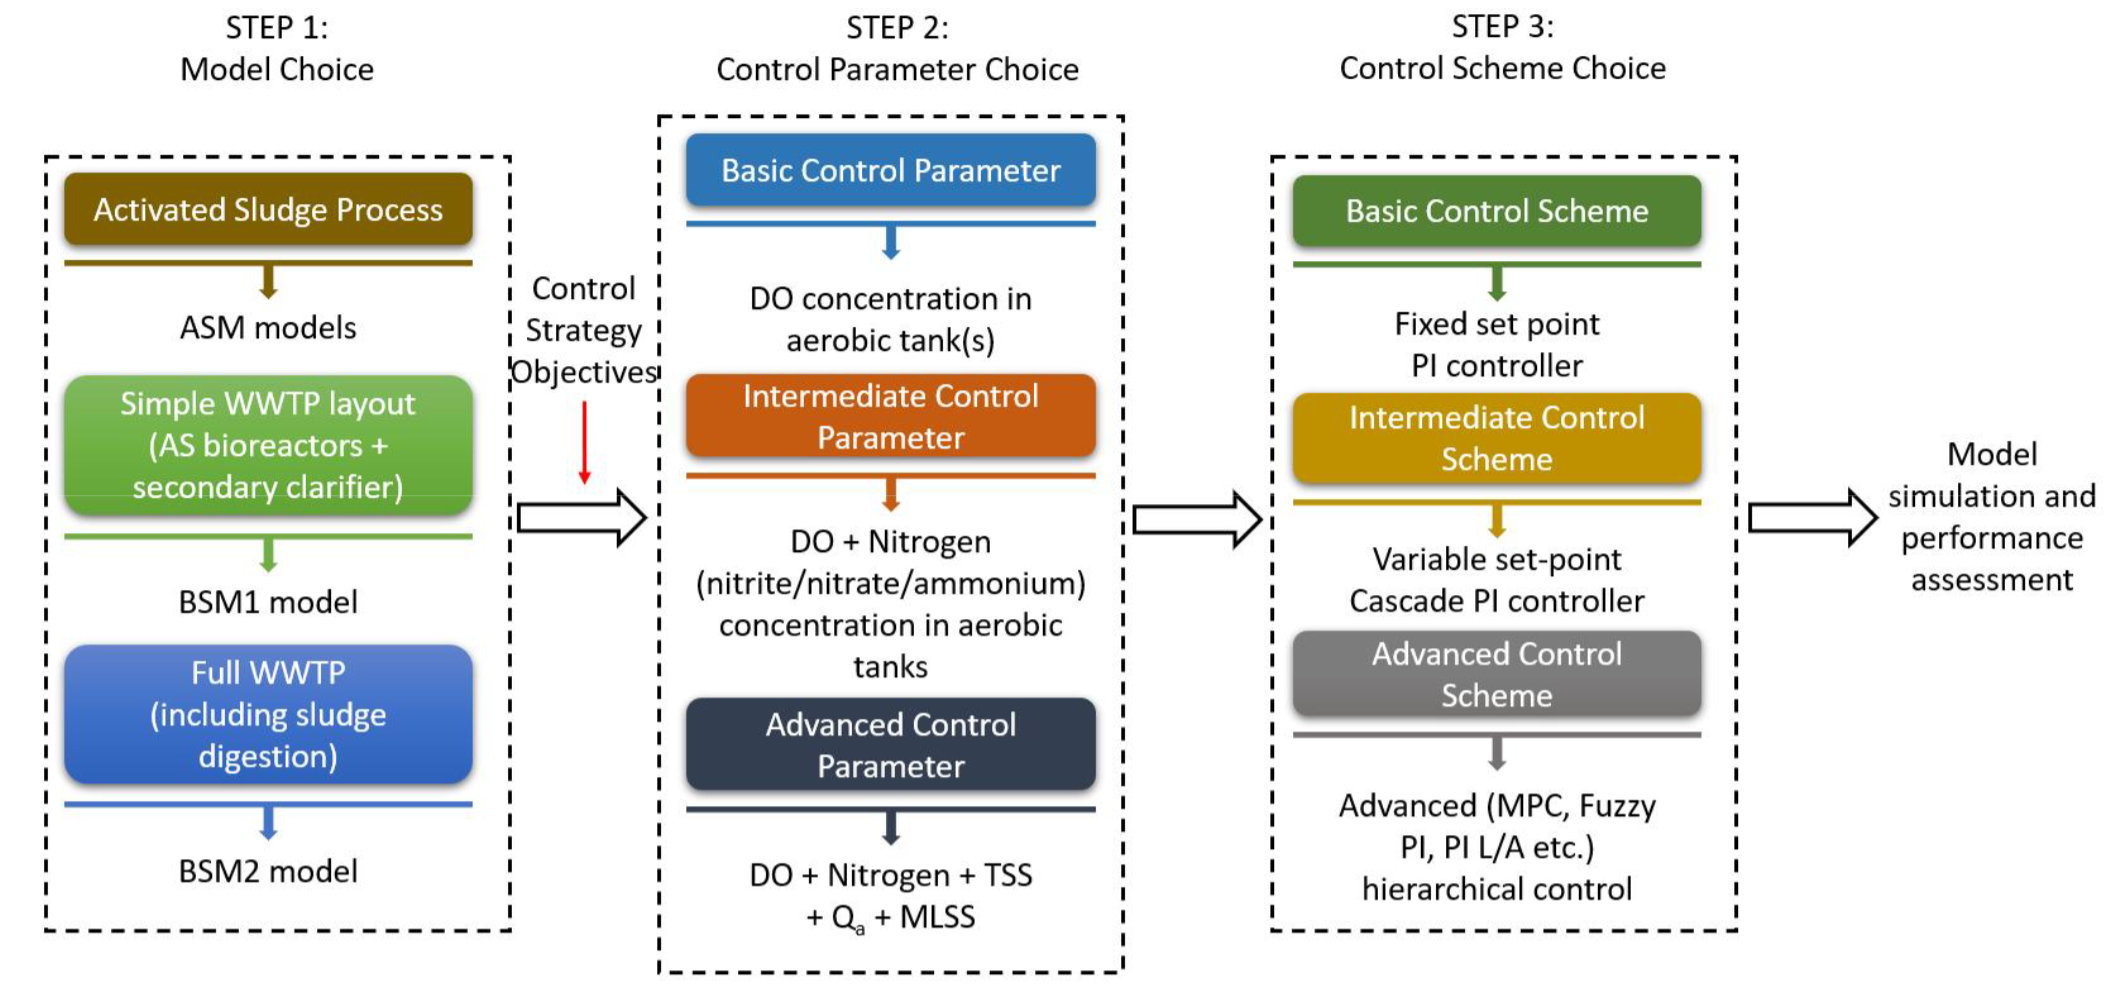
\includegraphics[width=0.9\columnwidth]{imgs/propose-frameworks-for-control-strategy-design.png}
   \caption{Proposed framework for control strategy design by \citet{ballhysaWastewaterTreatmentPlant2020}.}
   \label{fig:control-strategy-design}
\end{figure}
 
In recent year, many publications present an interesting way to demonstrate how machine learning based model predicitve control (MPC) can outperfrom the conventional PID controller in WWTPs using BSM. The researchers use Matlab-Simulink to simulate the treatment processes in WWTPs while the block of PID controllers are swapped to machine learning models, and the effluent quality or treatment system performance can be differentiated via BSM simulated results. \citet{wangModelPredictiveControl2020} compared the stability of chlorinated water quality in the effluent of a DWTP with two control strategies, which are PID feedback controls and a predictive model based support vector machine (SVM). The BSM simulated results showed the SVM model required 21 minutes less to reach the residaul chlorine setpoint compared to PID feedback controls. A proposed neuro-fuzzy PID controller (i.e., a hybrid machine learning model consisted of nerual networks and fuzzy logic) also showed a superior performance in optimizing the chlorine dosing rate and to minimize the chance of errors \citep{hongApplicationNeurofuzzyPID2012} The significance of using BSM in Matlab-Simulink enables the performance of traditional and machine learning based control strategies can be compared in objective and fair senarios, also providing the practicability of machine learning to the experts in the field. Matlab is a powerful and resourceful platform providing various machine learning functions, including point-and-click apps for training and evaluation, available algorithms of classification and regression algorithms, and Automatic machine learning (AutoML), etc \citep{mathworksMATLABMachineLearning2022}. The direct access to the abundant features along with the integration of Simulink makes Matlab an appealing option for many researchers in wastewater treatment industry, especially in the research domain in machine learning and control strategy simulation. Despite the countless benefits of using Matlab, Python programming language stands out in different ways.

Python is a high-level, interpreted, and object-oriented programming language, and features with simple and easy to learn syntax providing good readability \citep{WhatPythonExecutive}. The large developer community (e.g., GitHub and Stackoverflow) and open-source access (i.e., free of charge) have made Python an ideal tool for machine learning starters. The most cutting-edge research in the field of Artificial Intelligence is often led by the Tech Giants like Google and Amazon, which conduct research on Python (e.g., machine learning frameworks of TensorFlow (Google)in Python), as well as the big research community using Python. All the lasted updates and developments relating to machine learning architectures and techniques are usually accessible in open-source Python community, including the example codes. Contrary to Python, users on commercial software Matlab need to wait for the software engineers working in Matlab to update the lastest machine learning applications onto Matlab plaform, which is a time consuming process and create a delay of time and accessibilities to many resources \citep{castroWhyShouldChoose2018}. Machine learning developers in wastewater treament industry can freely choose between the programming methods based on the research need. For those looking for mature machine learning algorithms can simple use Matlab and be satisfied with the functionalities, on the other hand, for those intend to incoporate more new techniques and architecutures in machine learning model can consider using Python as the programming language. Interestingly, MathWorks recently announced using Python functions in Simulink Model \citep{mathworksCallPythonFunction2022}, despite the update from Matlab, to the best of my knowledge, there is no research papers develop machine learning on Python and run on Matlab-Simulink. 

\subsection{Data pre-processing}
The ubiquitous sensors installed in WWTPs for treatment automation generate a massive amount of data on daily basis. Before being used for any purposes, the data must be understandable for explanation and relevant enough for water experts to extract valuable information \citep{kehreinCriticalReviewResource2020}. Without the help of Artificial Intelligence, data manipulation before training machine learning models can be time-consuming and challenging. The specific designed algorithms can perform data evaluation and augmentation, thus the quality of data can be improved. Any statistical or machine leranign algorithms which can complete these tasks are known as the data pre-processing methods. The causes of sensors rendering undesired data with low quality are from the limitations of the hardware sensors and the dynamics of the sampling locations. In general, the fouing data generated by sensors can be described in eight distinct states \citep{rosenAddingRealismSimulated2008,newhartDatadrivenPerformanceAnalyses2019}:

\noindent
\begin{myenumerate}
    \item Operational: Sensor is working properly with normal measurement noise.
    \item Excessive drift: When a sensor outputs a value progressively further from the truevalue.
    \item Shift: When the output of the sensor is a constant amount away from its true value.
    \item Fixed value: When the sensor is stuck and keeps repeating the same value.
    \item Complete failure: Similar to a fixed value fault, but the sensors either give offthemaximum or minimum, value, zero or no value at all.
    \item Wrong gain: When signals away from the calibration point are under- orover-amplified bythe sensor.
    \item Calibration: The sharp change in sensor output directly following a calibration.
    \item Isolated fault: When a single point in a series shows an incorrect value.
\end{myenumerate}

The researchers and experts have been proposing solutions for filling the data gaps created from sensor faults and maintenance operations, but number and length of missing values are largely subject to the dynamics of the system being monitored and other factors. In their open-source wastewater data treatment toolkit,\citet{demulderOpenSoftwarePackage2018} has recommended five data inputation strategies aimed at data generated from water resource recovery facilities:

\noindent
\begin{myenumerate}
    \item Interpolate.
    \item Use a correlation with other available measurement signals.
    \item Replace with a corresponding value in an average daily profile.
    \item Repeat the values obtained on the preceding day.
    \item Replace with the output of a model. 
\end{myenumerate}

The efficient monitoring of sensors and proper use of the data for developing control strategies in wastewater treatment industry rely on careful data quality control. In recent years, the automated data evaluation has drawn attentions of experts and reseraches in this field while manually detection of sesor fouling is unrealistic due to the tasks are labor-intensive and laborious. \citet{alferesValidatingDataQuality2013} presented three practical approaches for data quality validation, which are capable of automated calculate single abnormal vaules and collective faults over a long period of time. The author claimed that the significance of the research work is performing data quality validation scheme on multivariate dataset. The pitfalls of the study is despite the promising approaches proposed in the study, the validity still depend on the thresholds or acceptability limits in the actaull WWTPs. Similar to the data inputation strategies, the real situation differs tremendously across different WWTPs. That being said, instead of providing general guidance of how to munipulate data, the focus should be emphasized on how to use algorithms to help users understand, analyze, and process the fouling data.

\subsection{Feature engineering}
The purpose of feature engineering aims at enriching the raw dataset through selecting, manipulating, and transforming data, which forms better dataset relating to the underlying targets to be learning by the machine learning model. Feature engineering and data pre-processing are easily confused with each other, the fundamental difference between the two is the former creates actual features which are not included in the raw data, while the latter is a data noise removing and cleaning process. In the study of \citet{mamandipoorMonitoringDetectingFaults2020}, feature engineering was performed to generate five extra features, which are the statistical metrics of mean, maximum, minimum, variance and standard deviation of a specific input feature. However, in the comparisons of the final results, the author only emphasized on evaluating model accuracies across varied machine learning models (i.e, PCA-SVM and LSTM models). Another interesting technique used by \citet{zaghloulDevelopmentEnsembleMachine2021} is to create the gradient values of an input variable to assist the model to better learn the trend of the historical removal rate of water parameters in aerobic granular sludge reactors. Similar to the results showed in the work of \citet{mamandipoorMonitoringDetectingFaults2020}, the influence of how engineered features affects the ultimate model accuracy is excluded in the results and discussion part. This raises many questions like how significant the feature engineered inputs are to the model accuray, and which techniques can be used upon which senarios. 

There is still a considerable ambiguity with regard to the neccessity of using feature engineered inputs in traning predictive model in WWTPs. In the prediction of total nitrogen (TN) in the effluent, the author input nine features and performed feature sensitivity analysis, which can capture the change of the output values attributed to the change input. The result showed that the top three most significant inputs, which are temperature, TN flow and pH share significant effectiveness to the prediction of TN. The author claimed physical related cause-and-effect relationships bewteen the effluent TN and those top three effecitve features can be elucidated by machine learning model \citep{guoPredictionEffluentConcentration2015}. In another work of predicting influent BOD concentration, the study clearly stated using five inputs instead of three inputs will cause model overfitting, and three inputs for model training was considered sufficient citep{Alsulaili}. Varaibles that are created from feature engineering have no physical properties, leading to extra unexplainable essence in addition to the black box nature of machine learning models. Besides, extra model inputs from feature engineering can also cause overfitting if the data quality is not carefully evaluated. Said by Andrew Ng, "Coming up with features is difficult, time-consuming, requires expert knowledge. Applied machine learning is basically feature engineering". From the quote and the recent studies we are uncertain to how feature engineering techniques can practically help the development of machine learning models in wastewater treatment industry, more research is required to futher elucidate the effectiveness of performing feature engineering.